\documentclass[12pt]{article}
	
\usepackage[margin=1in]{geometry}		% For setting margins
\usepackage{amsmath}				% For Math
\usepackage{fancyhdr}				% For fancy header/footer
\usepackage{graphicx}				% For including figure/image
\usepackage{cancel}					% To use the slash to cancel out stuff in work

%%%%%%%%%%%%%%%%%%%%%%
% Set up fancy header/footer
\pagestyle{fancy}
\fancyhead[LO,L]{Chengming Li}
\fancyhead[CO,C]{ECE257a - Homework1 }
\fancyhead[RO,R]{\today}
\fancyfoot[LO,L]{}
\fancyfoot[CO,C]{\thepage}
\fancyfoot[RO,R]{}
\renewcommand{\headrulewidth}{0.4pt}
\renewcommand{\footrulewidth}{0.4pt}
%%%%%%%%%%%%%%%%%%%%%%


\begin{document}
%%%%%%%%%%%%%%%%%%%%%%%% Q1
\noindent \textbf{Problem 1 (5pt). Explain why the Internet adopts a hierarchical architecture. Does the modern Internet strictly follow a tree structure? Explain your answer.\\}


\textbf{Answer:} Hierarchical architecture (divide and conquer) achieves scalability. Having such architecture means every access net can connect to various ISPs(it doesn't need to be single one, or a global one). And it also reduces the complexity of the Internet network. Imagine if we have N access net, we need $N^2$ connections to have them all connected, and sometimes it is not necessary to have those connections. \\
\indent The modern Internet does not strictly follow a tree structure because modern communication is looking for low-latency data communication. Part of the network is flattened out because of this reason to achieve faster communication and local data processing. On the other hand, some interconnection points may need to have contact with other ISPs, or Internet exchange points, or regional nets, etc. And those points may not share the same path as the interconnection points. \\

%%%%%%%%%%%%%%%%%%%%%%%% Q1 END



%%%%%%%%%%%%%%%%%%%%%%%% Q2
\noindent \textbf{Problem 2 (10pt). Quickly study the SoftRAN and SoftCell papers listed in the reference part of Lecture 02. Answer the following questions:}\\
\begin{itemize}
    \item What benefits does software defined networking bring to cellular networks? Provide
sufficient details to support your answer. 
    \item Think of one more example scenario where software defined wireless networks are
superior to conventional wireless network architectures. Explain your idea. Use the hints
from the papers but do not use their existing examples directly
\end{itemize}



\textbf{Answer:}
\begin{itemize}
    \item Based on “SoftRAN: Software Defined Radio Access Network”, ACM HotSDN’13, software-defined networking can "perform load balancing and interference management, as well as maximize for throughput,
global utility." And these goals are suboptimal in the LTE’s current distributed control plane due to the high complexity and density of wireless infrastructure. Regarding the workload reduction in the control pannel, this paper addresses two principles: 1. All control decisions that influence the decision making
at neighboring radio elements must be made at the controller since such decisions need to be coordinated
across radio elements.2. All decisions that are based on frequently varying parameters should preferably be made at the radio element, since the inherent delay between the radio element and the controller increases the response time to these frequently varying parameters. These two principles aim to reduce the workload of the local controller and the delay between the radio element and the controller.
    \item One example I can think of is the "Public Free Wifi" in the public building. One common scenario is the stability of this "WIFI". People may lose the connection very quickly and unintentionally and get their connection back after a while. This is due to the management of load balance in the software-defined wireless networks. The control panel aims to balance the load distribution to avoid the heavy traffic in one single access point so that the user experience is enhanced. \\
\end{itemize}

%%%%%%%%%%%%%%%%%%%%%%%% Q2 END



%%%%%%%%%%%%%%%%%%%%%%%% Q3
\noindent \textbf{Problem 3 (5pt). Review the Web request example we went through in Lecture 3. Suppose
instead of Web browsing, the user opens a YouTube video on her smartphone. Describe the
network entities (e.g., application service providers, ISPs, etc.) and devices involved in this
procedure, and also describe their work flow. List the major network protocols and briefly
explain their roles. Think of as many protocols as you can.\\}


\textbf{Answer:}
\begin{itemize}
    \item Network discovery and association: Wifi Ap keeps broadcasting beacons with the user's smartphone MAC address. The client listens and sends association request. Then, the client connects to WIFI IP.
    \item IP address allocation: the smartphone client needs to get its own IP address, addr of first-hop router, addr of DNS server. All done using DHCP(Dynamic Host Configuration Protocol). The role of DHCP is: responds client's request and allocates an IP address to it.
    \item DNS request: Map www.youtube.com to its IP address through database and route the request to DNS server.
    \item Routing DNS request: ask first-hop router to route the request and cliend need to communcate with first-hop router by knowing its MAC address, done by ARP(address resolution protocol)
    \item Sending DNS request: 1. client creates an IP packet containing DNS request, which goes to first-hop router. 2. Router forwards packet from campus network to Comcast network to DNS server, following Internet routing protocol. 3. DNS server replies to the client with the IP address of www.youtube.com.
    \item Establish TCP flow: Client creates a TCP flow to Web server.
    \item Getting Youtube video:, clients sedn HTTP request through the TCP flow, server sends the Youtube videos page back to client.\\
\end{itemize}

%%%%%%%%%%%%%%%%%%%%%%%% Q3 END



%%%%%%%%%%%%%%%%%%%%%%%% Q4
\noindent \textbf{Problem 4 (9pt). Understand wireless network performance metrics.\\}
\begin{enumerate}
        \item Does higher network throughput always mean lower latency? Why?
        \item Why higher network density improves per-user link capacity in general? Will the total
capacity of a wireless network keep increasing if more and more basestations are
deployed in the same area?
        \item Given the same bandwidth (spectrum width), will a high-frequency communication link
(e.g., 5G mmWave link) always achieve a higher bit-rate than a low-frequency
communication link (e.g., WiFi link)?
\end{enumerate}

\textbf{Answer:}
\begin{itemize}
    \item High throughput doesn't necessarily mean low latency. Latency is the combination of the transmission delay + propagation delay + queuing delay. Let's imagine we are sending lots of packets of information from Boston to San Diego. The propagation delay is heavily increased due to the distance between northeast to southwest, the transmission delay may also increase due the lower link capacity because they are not the major city in ease and west coast., and lastly, the queuing delay is heavily increased as well due to the number of hubs, intermediate connection delay and packet processing.
    \item  Higher network density means lower load in each network station and better signal quality as lower interference. With more network stations, per-user can get better service as they are the only ones using it. It is like the difference when 1 cake is shared by 10 people and 1 cake is shared by 1 person. In reality, the total capacity of a wireless network will not keep increasing linearly due to the limited spectrum bandwidth and network station infrastructure.
    \item This is not always true. Several factors affect performance, such as distortion, network traffic, and user environment etc. Distortion can be hard to deal with when in the high-frequency and it takes time to sort out the baseband information. We couldn't say the higher-frequency communication link always achieves a higher bit-rate than a low-frequency communication link if the network traffic is heavy and there are multiple active users.\\
\end{itemize}

%%%%%%%%%%%%%%%%%%%%%%%% Q4 END



%%%%%%%%%%%%%%%%%%%%%%%% Q5
\noindent \textbf{Problem 5 (15pt). Understand wireless propagation.\\}
\begin{enumerate}
    \item Does wireless signal strength always get weaker as link distance increases? Why?
    \item Suppose a 30 GHz transmitter and a 3 GHz transmitter send signals at the same power
level, estimate the difference between the received signal power (assuming link distance
and antenna gains are the same).
    \item Suppose a transmitter increases its transmit power by 10 dB, how will the transmission
range increase? How about 3 dB? (Provide a coarse estimation.)
    \item How does multipath reflection cause frequency-selective fading (i.e., channel gain
various across different frequencies)?
    \item Coherence time is a metric to quantify how stable the wireless channel over time.
Intuitively, it is a time-domain metric. But why is it related to the Doppler shift which is
a frequency-domain metric?
 
\end{enumerate}


\textbf{Answer:} 
\begin{itemize}
    \item Yes, based on the Free-space pathloss model, the received signal power is proportional to $\frac{1}{d^2}$. And there are several effects that happen during signal propagation: Pathloss(attenuation) over distance, Multipath effect, and Temporal variation.
    \item Again, based on the Free-space pathloss model($P_{r} = G_{r}G_{t}(\frac{\lambda}{4\pi d})^2P_{t}$), 30G Hz has shorter wavelength than 3G Hz so that it suffers more from pathloss.
    $\frac{P_{r 30Ghz}}{P_{r3Ghz}} =\frac{(3e8/30e9)^2}{(3e8/3e9)^2} =\frac{0.01^2}{0.1^2}$
    \item Starting from 3dB, every 3dB power increase results in doubling the power. And $d = \frac{1}{\sqrt{P_r}}$ In order to compensate the 3 dB power increase, the distance needs to be $\sqrt{2}$d longer. 10dB increase results in 8x-9x power, The distance will increase around 2.8d - 3d longer.
    \item Multipath's copies can either strengthen or weaken each other, depending on whether they are in or out of phase. For a given receiver location, whether two waves are in or out of phase depends on frequency. So at some frequency, the copies are out of phase with each other and cause the signal to be extremely weak(Deep fading regions).
    \item Based on the Empirical model, the coherence time also depends on movement speed as $T_{c} = \frac{9}{16 \pi f_{d}} = \frac{9}{16 \pi vf}$. This is created by the movement of the transmitter, receiver, or objects in the environment\\
\end{itemize}

%%%%%%%%%%%%%%%%%%%%%%%% Q5 END



%%%%%%%%%%%%%%%%%%%%%%%% Q6
\noindent \textbf{Problem 6 (6pt). DSSS modulation.\\}
\begin{enumerate}
    \item Explain how DSSS modulation improves the link SNR compared with the case without
spreading.
    \item Explain how DSSS modulation realizes 250 Kbps bit rate over a 2MHz channel for
ZigBee, and how it realizes 1 Mbps bit rate over a 22 MHz channel for 802.11b.
\end{enumerate}

\textbf{Answer:} 
\begin{itemize}
    \item DSSS uses spread spectrum modulation to convert a narrowband signal into a wideband symbol. In the receiver side, the noise is also spread by the DSSS(especially the narrowband interference) $\xrightarrow{}$ Lower Noise. Thus, it increases the SNR by lowering the noise.\\
    In the case without spreading, the narrowband interference heavily affects the SNR, and the SNR increase.
    \item In ZigBee, every 4 bits is converted into one symbol (250kb/s / 4 = 62.5kS/s). And every symbol is spreading out by factor 32 (62.5kS/s * 32 = 2 MChips/s) Every I or Q signal takes 0.5us(1/0.5us = 2M Hz bandwidth)\\
    In 802.11b, each bit is spread using a chip sequence(length = 11) called Barker code. 1Mbps bit = 11Mhz chip rate. But there are 2 samples(I and Q) in each chip, so the sampling rate is 11Mhz *2 = 22 Mhz as the bandwidth. In order to receive the information of I and Q, the bandwidth and sampling rate needed to be 22Mhz.\\
\end{itemize}

%%%%%%%%%%%%%%%%%%%%%%%% Q6 END

\noindent \textbf{Problem 7 (6pt). DSSS modulation.\\}
(1)\\
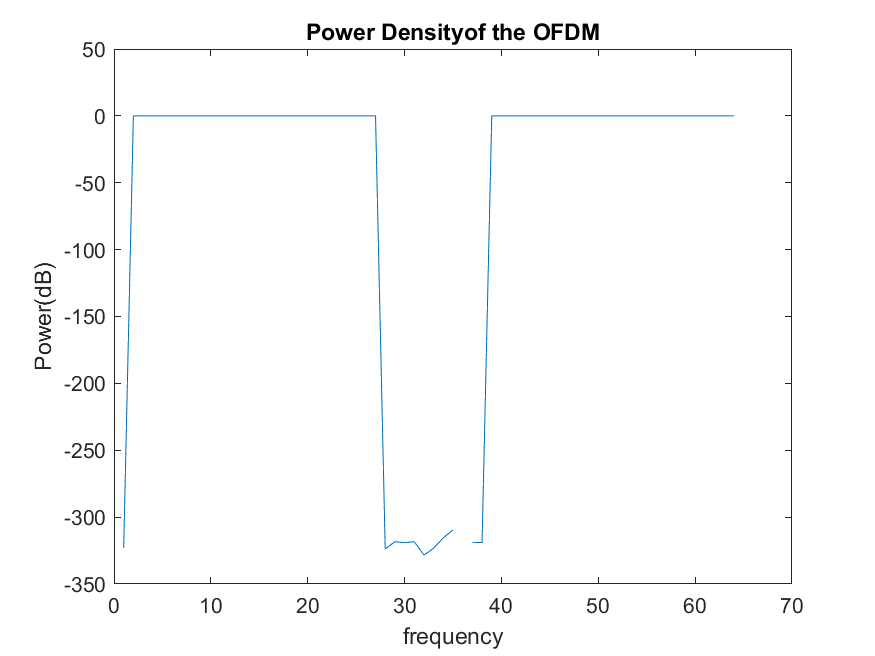
\includegraphics[scale=0.8]{Power_Spectrum_Density.png}\\
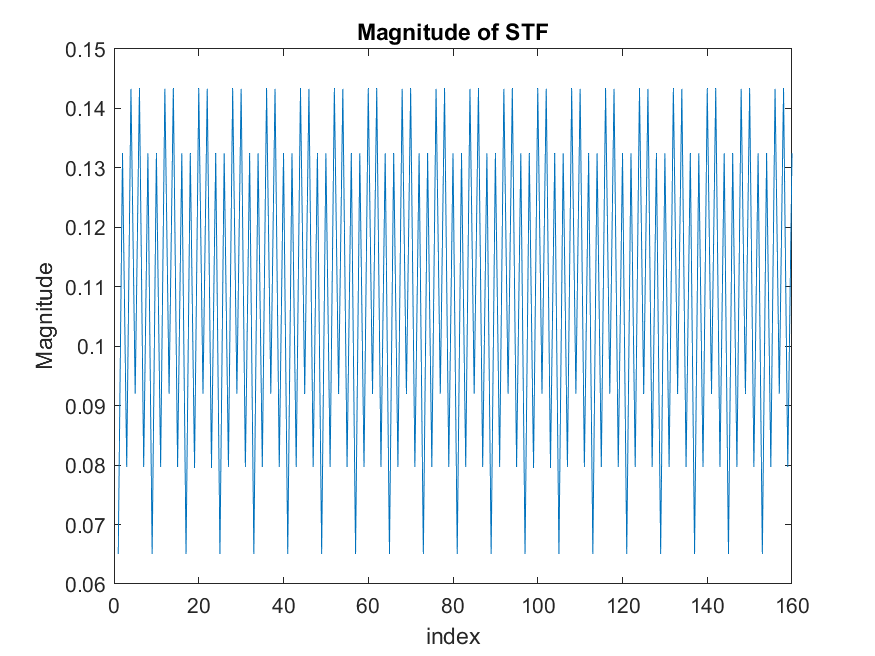
\includegraphics[scale=0.8]{Magnitude of STF.png}\\
(2)\\
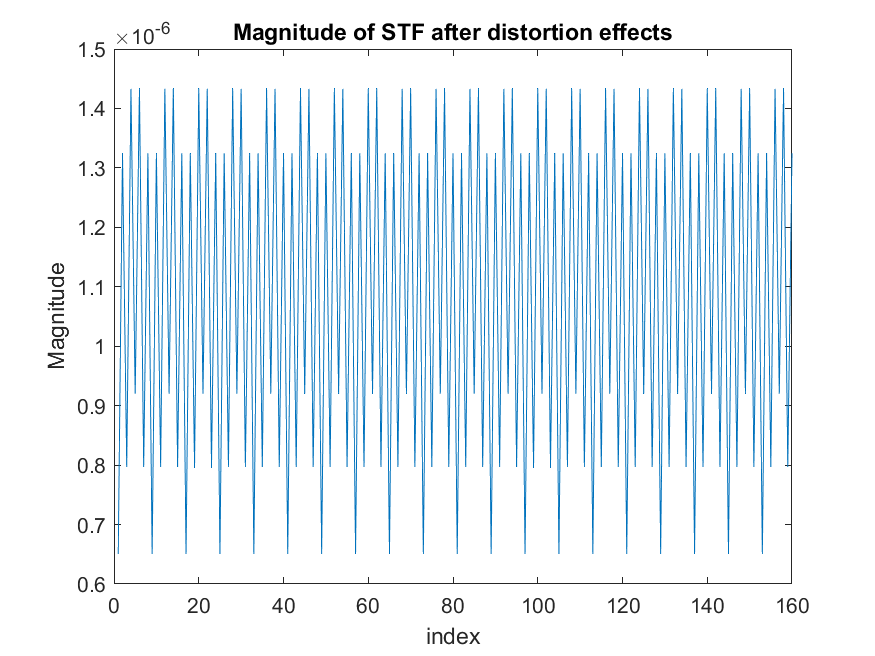
\includegraphics[scale=0.8]{Magnitude_of_STF_after_distortion_effects.png}\\
(3)\\
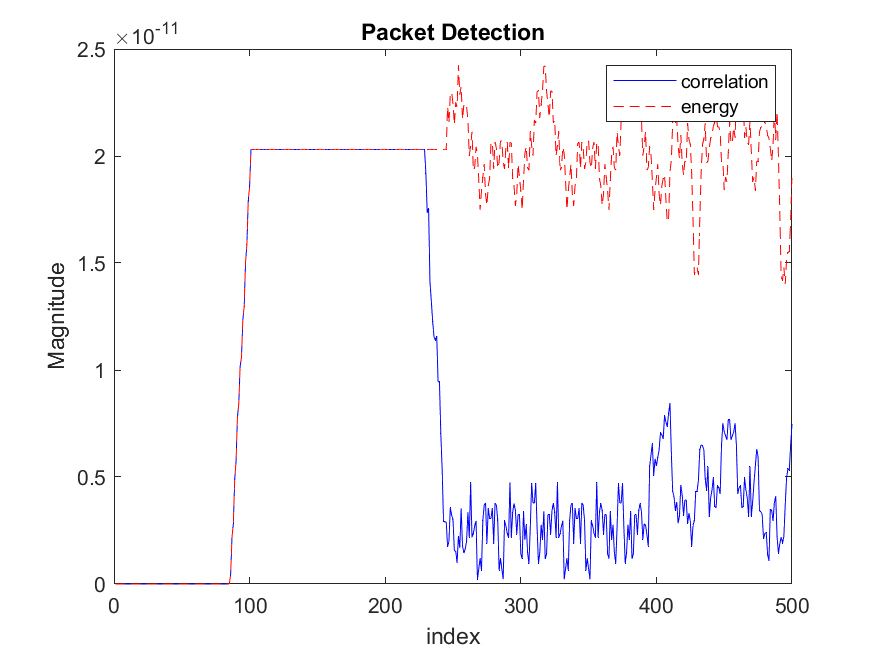
\includegraphics[scale=0.8]{Packet_Detection.png}\\
Index of the samples where packets are detected: 101-260\\
(4)\\
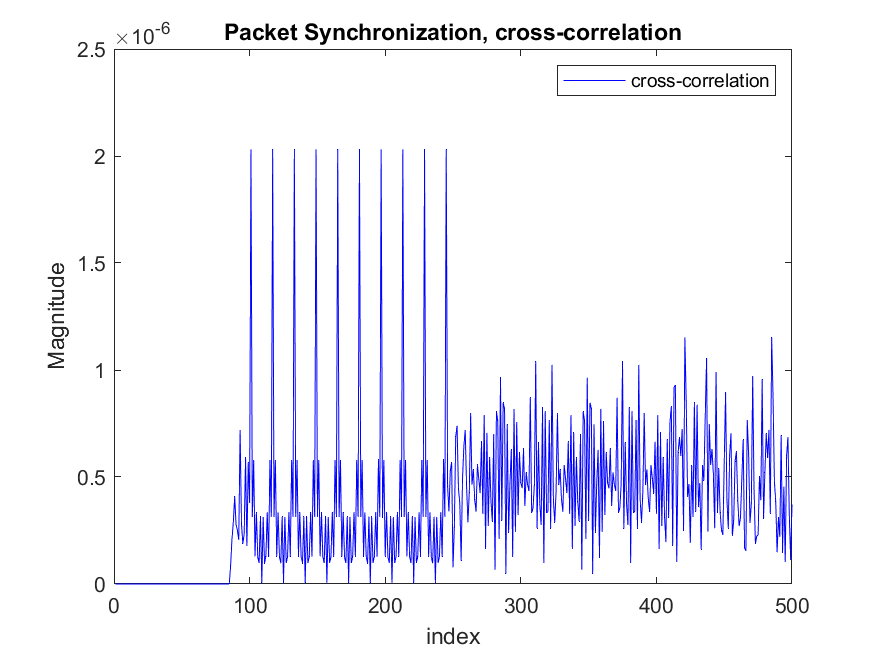
\includegraphics[scale=0.8]{Packet-Synchronization_cross-correlation.png}
indices of samples corresponding to the STF starting time: 101   117   133   149   165   181   197   213   229   245\\
(5)\\
Frequency offset: 1.6987e-04\\
All print out results can be seen in the scripts.
\end{enumerate}
\end{document}